\documentclass[12pt,a4paper]{article}

% ==================================================
% PENGATURAN HALAMAN & MARGIN STANDAR FMIPA UNS (4-3-4-3 cm)
% ==================================================
\usepackage[
  a4paper,
  top=4cm,
  bottom=3cm,
  left=4cm,
  right=3cm,
  headsep=2.0cm,
  footskip=1.5cm,
  headheight=15pt
]{geometry}

\usepackage{fancyhdr}
\pagestyle{fancy}
\fancyhf{}
\fancyfoot[C]{\thepage}
\renewcommand{\headrulewidth}{0pt}
\renewcommand{\footrulewidth}{0pt}

\fancypagestyle{plain}{
  \fancyhf{}
  \fancyfoot[C]{\thepage}
  \renewcommand{\headrulewidth}{0pt}
  \renewcommand{\footrulewidth}{0pt}
}

% ==================================================
% FONT, SPASI, DAN PARAGRAF
% ==================================================
\usepackage{mathptmx} % Times New Roman
\usepackage{setspace}
\setstretch{1.42} % Spasi 1.5 standar
\setlength{\parindent}{1.25cm}
\setlength{\parskip}{0pt}
\setcounter{secnumdepth}{3}

% ==================================================
% LINGKUNGAN MATEMATIKA
% ==================================================
\usepackage{amsmath,amssymb,amsfonts,amsthm}
\numberwithin{equation}{section}
\renewcommand{\theequation}{\arabic{section}.\arabic{equation}}

\AtBeginDocument{
  \setlength{\abovedisplayskip}{3pt}
  \setlength{\belowdisplayskip}{3pt}
  \setlength{\abovedisplayshortskip}{1pt}
  \setlength{\belowdisplayshortskip}{1pt}
}
\allowdisplaybreaks

% ==================================================
% GAMBAR, TABEL, DAN FORMAT LAINNYA
% ==================================================
\usepackage{graphicx}
\usepackage{booktabs}
\usepackage{array}
\usepackage{float}
\usepackage[labelsep=period, justification=centering]{caption}
\usepackage{subcaption}
\usepackage{cite}
\usepackage{enumitem}
\usepackage[hidelinks]{hyperref}
\usepackage{microtype}
\usepackage{listings}
\usepackage{xcolor}

\setlist[enumerate,1]{label=\arabic*., nosep, leftmargin=0.75cm}
\setlist[enumerate,2]{label=\alph*., nosep, leftmargin=0.55cm}
\setlist[itemize]{nosep, leftmargin=0.55cm}

% Penyesuaian bahasa Indonesia sesuai Pedoman S1 Matematika UNS
\usepackage[indonesian,provide=*]{babel}
\addto\captionsindonesian{%
  \renewcommand{\figurename}{Gambar}%
  \renewcommand{\tablename}{Tabel}%
  \renewcommand{\refname}{DAFTAR RUJUKAN}%
  \renewcommand{\appendixname}{LAMPIRAN}%
}

% Format Daftar Rujukan yang rapi dan proporsional (Model Plain)
\let\oldthebibliography\thebibliography
\let\endoldthebibliography\endthebibliography
\renewenvironment{thebibliography}[1]{%
  \begin{oldthebibliography}{#1}%
    \thispagestyle{plain}%
    \setlength{\itemsep}{2pt}%
    \setlength{\parsep}{0pt}%
    \setlength{\parskip}{0pt}%
}{%
  \end{oldthebibliography}%
}

% Format Listing Kode
\lstset{
  basicstyle=\ttfamily\scriptsize,
  breaklines=true,
  frame=single,
  numbers=left,
  numberstyle=\tiny\color{gray},
  keywordstyle=\color{blue}\bfseries,
  commentstyle=\color{green!50!black}\itshape,
  stringstyle=\color{red!70!black},
  showstringspaces=false,
  tabsize=2,
  backgroundcolor=\color{gray!5}
}

% ==================================================
% FORMAT JUDUL BAB DAN SEKSI
% ==================================================
\usepackage{titlesec}

% Format Bab (Angka Romawi: BAB I, BAB II, dst.)
\renewcommand{\thesection}{\Roman{section}}
\titleformat{\section}[display]
  {\centering\bfseries}
  {\fontsize{14pt}{16pt}\selectfont BAB \thesection}
  {0.15cm}
  {\fontsize{14pt}{16pt}\selectfont}
\titlespacing*{\section}{0pt}{0.3em}{0.6em}

% Format Subbab
\renewcommand{\thesubsection}{\arabic{section}.\arabic{subsection}}
\titleformat{\subsection}[block]
  {\bfseries\normalsize}
  {\thesubsection}
  {0.4em}
  {}
\titlespacing*{\subsection}{0pt}{0.35em}{0.12em}

% Format Anak Subbab
\renewcommand{\thesubsubsection}{\arabic{section}.\arabic{subsection}.\arabic{subsubsection}}
\titleformat{\subsubsection}[block]
  {\bfseries\normalsize\itshape}
  {\thesubsubsection}
  {0.4em}
  {}
\titlespacing*{\subsubsection}{0pt}{0.25em}{0.08em}

% ==================================================
% AWAL DOKUMEN
% ==================================================
\begin{document}

% --------------------------------------------------
% HALAMAN JUDUL (COVER RESMI)
% --------------------------------------------------
\begin{titlepage}
  \thispagestyle{empty}
  \begin{center}
    \setstretch{1.3}
    {\fontsize{14pt}{17pt}\selectfont\bfseries
    LAPORAN PENGANTAR PROSES STOKASTIK\par}
    \vspace{0.4cm}
    {\fontsize{13pt}{16pt}\selectfont\bfseries
    PEMODELAN RANTAI MARKOV ABSORBING STATE PADA DINAMIKA TRANSISI STATUS INFEKSI COVID-19 DI INDONESIA\par}
    
    \vspace{1.2cm}
    
\includegraphics[width=4.6cm]{logo_uns.png}
    \vspace{1.2cm}
    
    {\fontsize{12pt}{14pt}\selectfont\bfseries Dosen Pengampu:\par}
    \vspace{0.15cm}
    {\fontsize{12pt}{14pt}\selectfont Ade Susanti, S.Si., M.Si.\par}
    
    \vspace{1.0cm}
    {\fontsize{12pt}{14pt}\selectfont\bfseries Disusun Oleh:\par}
    \vspace{0.25cm}
    {\fontsize{12pt}{14pt}\selectfont
    \begin{tabular}{ll}
      Fadhila Hardi Ningrum           & (M0124004) \\
      Karunia Febyayu Puspitaningtyas & (M0124010) \\
      Ramadhan Imanur Rochim          & (M0124015) \\
      Achika Vigo Azhyra              & (M0125001) \\
      Fawwaz Absyar Rifai             & (M0125044)
    \end{tabular}\par}
    
    \vfill
    {\fontsize{12pt}{14pt}\selectfont\bfseries
    PROGRAM STUDI MATEMATIKA\\
    FAKULTAS MATEMATIKA DAN ILMU PENGETAHUAN ALAM\\
    UNIVERSITAS SEBELAS MARET\\
    2026\par}
  \end{center}
\end{titlepage}

\newpage
\pagenumbering{arabic}
\setcounter{page}{1}

% --------------------------------------------------
% BAB I: PENDAHULUAN
% --------------------------------------------------
\section{PENDAHULUAN}
\thispagestyle{plain}

\subsection{Deskripsi Fenomena Nyata}
Penyebaran penyakit menular seperti COVID-19 melibatkan perubahan status kesehatan individu dalam populasi dari waktu ke waktu. Dinamika ini sering dimodelkan melalui pendekatan epidemiologi kompartemen. Namun, model kompartemen diferensial deterministik memiliki kelemahan berupa sensitivitas yang tinggi terhadap fluktuasi parameter laju penularan. Sebagai pendekatan stokastik alternatif, Zhang dkk. \cite{zhang2020} menunjukkan bahwa Rantai Markov Waktu Diskret (\textit{Discrete-Time Markov Chain}) dapat digunakan untuk memodelkan pergerakan status individu berdasarkan data pengamatan harian secara langsung.

Karakteristik penting dalam dinamika infeksi COVID-19 adalah keberadaan keadaan penyerap (\textit{absorbing state}). Status Sembuh dan Meninggal Dunia bertindak sebagai keadaan penyerap alami, karena individu yang telah meninggal dunia tidak dapat berpindah ke status lain. Demikian pula dalam kurun waktu pengamatan tertentu, individu yang telah sembuh diasumsikan memiliki antibodi protektif sehingga tidak tertular kembali dalam periode model. Teori rantai Markov hingga dengan keadaan penyerap serta analisis langkah pertama (\textit{First Step Analysis}) mengacu pada karya Kemeny dan Snell \cite{kemeny1976}, Taylor dan Karlin \cite{taylor1998}, serta Ross \cite{ross2014}.

\subsection{Sumber Data dan Asumsi Eksplisit}
Data empiris yang dianalisis merupakan data deret waktu harian kasus COVID-19 di Indonesia periode 2 Maret 2020 hingga 16 September 2022 (929 hari kalender) yang dikompilasi oleh Hendratno \cite{hendratno2022}, bersumber resmi dari Satuan Tugas Penanganan COVID-19 \cite{satgascovid2022} dan Kementerian Kesehatan Republik Indonesia \cite{kemenkes2020}. Asumsi yang digunakan meliputi (1) populasi bersifat tertutup dengan jumlah penduduk konstan $N = 265.185.520$ jiwa, (2) status Sembuh dan Meninggal Dunia merupakan keadaan penyerap sempurna, serta (3) peluang transisi antarstatus bersifat homogen terhadap waktu selama masa pengamatan.

\subsection{Definisi Proses Stokastik dan Klasifikasinya}
Didefinisikan variabel acak $X_n$ sebagai status kesehatan seorang individu representatif pada hari ke-$n$. Ruang keadaan (\textit{state space}) didefinisikan sebagai
\[
  S = \{S, I, R, D\},
\]
dengan $S$ (\textit{Susceptible}) adalah individu rentan yang berisiko terinfeksi, $I$ (\textit{Infected}) adalah individu yang terinfeksi aktif, $R$ (\textit{Recovered}) adalah individu yang telah sembuh, dan $D$ (\textit{Death}) adalah individu yang meninggal dunia akibat COVID-19.

Indeks waktu didefinisikan sebagai
\[
  T = \{0, 1, 2, 3, \dots\},
\]
dengan indeks $n$ merepresentasikan hari pengamatan ke-$n$. Berdasarkan ruang keadaan dan indeks waktu yang bersifat diskrit, proses ini diklasifikasikan sebagai Rantai Markov Waktu Diskret (\textit{Discrete-Time Markov Chain}) yang memenuhi sifat Markov
\begin{equation}
  \Pr(X_{n+1} = j \mid X_n = i, X_{n-1} = i_{n-1}, \dots, X_0 = i_0) = \Pr(X_{n+1} = j \mid X_n = i) = P_{ij}.
  \label{eq:markov_property}
\end{equation}
Sesuai persamaan (\ref{eq:markov_property}), peluang proses berada pada keadaan $j$ pada hari berikutnya hanya bergantung pada keadaan $i$ pada hari ini, bukan pada riwayat hari sebelumnya.

% --------------------------------------------------
% BAB II: PEMBAHASAN
% --------------------------------------------------
\section{PEMBAHASAN}
\thispagestyle{plain}

\subsection{Penyusunan Peluang Matriks Transisi}
Berdasarkan data COVID-19 Indonesia periode 2 Maret 2020 sampai 16 September 2022, proses stokastik dibentuk dengan empat \textit{state}, yaitu $S$ (\textit{Susceptible}), $I$ (\textit{Infected}), $R$ (\textit{Recovered}), dan $D$ (\textit{Death}). Jumlah individu pada masing-masing \textit{state} ditentukan berdasarkan data harian dengan
\begin{align*}
  S_n &= N - \text{Total Cases}_n, \\
  I_n &= \text{Total Active Cases}_n, \\
  R_n &= \text{Total Recovered}_n, \\
  D_n &= \text{Total Deaths}_n,
\end{align*}
dan jumlah penduduk konstan $N = 265.185.520$.

Peluang transisi dihitung dari rasio perubahan jumlah individu pada masing-masing \textit{state} dengan menghitung rata-rata pada 929 hari pengamatan. Peluang perpindahan dari \textit{state} $S$ ke $I$ diperoleh melalui perbandingan kasus terbaru terhadap populasi rentan,
\begin{equation*}
  P_{SI} = \frac{\text{New Cases}}{S} = \frac{\sum P_{SI}}{929} = \frac{0{,}024450685}{929} = 0{,}000026319 \approx 0{,}000026.
\end{equation*}
Karena dari \textit{state} $S$ hanya terdapat dua kemungkinan, yaitu tetap berada di \textit{state} $S$ atau berpindah ke $I$, maka peluang individu yang berada pada kondisi rentan
\begin{equation*}
  P_{SS} = 1 - P_{SI} = 1 - 0{,}000026319 = 0{,}999973681 \approx 0{,}999974.
\end{equation*}
Kemudian, peluang perpindahan dari \textit{state} $I$ ke \textit{state} $R$ serta dari \textit{state} $I$ ke \textit{state} $D$ secara berturut-turut
\begin{equation*}
  P_{IR} = \frac{\text{New Recovered}}{I} = \frac{58{,}195056255}{929} = 0{,}062642687 \approx 0{,}062643,
\end{equation*}
\begin{equation*}
  P_{ID} = \frac{\text{New Deaths}}{I} = \frac{1{,}917890933}{929} = 0{,}002064468 \approx 0{,}002064.
\end{equation*}
Setelah nilai $P_{IR}$ dan $P_{ID}$ diketahui, peluang individu tetap berada pada \textit{state} $I$ dihitung melalui persamaan
\begin{equation*}
  P_{II} = 1 - P_{IR} - P_{ID} = 1 - 0{,}062643 - 0{,}002064 = 0{,}935293.
\end{equation*}
Pada model ini, \textit{state} $R$ dan $D$ ditetapkan sebagai \textit{absorbing state}, sehingga peluang untuk berada pada kondisi tersebut bernilai 1 ($P_{RR} = 1, P_{DD} = 1$), sedangkan peluang perpindahan dari ke \textit{state} lainnya bernilai 0. Berdasarkan urutan \textit{state} $(S, I, R, D)$, diperoleh matriks peluang transisi $P$ dengan struktur
\begin{equation}
  P = 
  \begin{pmatrix}
    P_{SS} & P_{SI} & P_{SR} & P_{SD} \\
    P_{IS} & P_{II} & P_{IR} & P_{ID} \\
    P_{RS} & P_{RI} & P_{RR} & P_{RD} \\
    P_{DS} & P_{DI} & P_{DR} & P_{DD}
  \end{pmatrix}
  =
  \begin{pmatrix}
    0{,}999974 & 0{,}000026 & 0 & 0 \\
    0          & 0{,}935293 & 0{,}062643 & 0{,}002064 \\
    0          & 0          & 1 & 0 \\
    0          & 0          & 0 & 1
  \end{pmatrix}.
  \label{eq:matrix_P}
\end{equation}
Dari struktur matriks $P$ pada persamaan (\ref{eq:matrix_P}), terlihat bahwa individu pada \textit{state} $S$ dapat tetap berada di $S$ atau berpindah ke $I$. Dari \textit{state} $I$, individu dapat tetap berada di $I$, berpindah ke $R$, atau berpindah ke $D$. Sedangkan \textit{state} $R$ dan $D$ bersifat menyerap karena memiliki peluang tetap sebesar 1.

\subsection{Verifikasi Syarat Matriks Stokastik}
Suatu matriks persegi $P$ merupakan suatu matriks peluang transisi apabila memenuhi dua syarat, yaitu setiap elemen matriks harus tidak negatif ($P_{ij} \ge 0$ untuk setiap $i, j$), kemudian jumlah peluang pada setiap baris harus bernilai 1.
\begin{align*}
  \sum_j P_{Sj} &= P_{SS} + P_{SI} + P_{SR} + P_{SD} = 0{,}999974 + 0{,}000026 + 0 + 0 = 1, \\
  \sum_j P_{Ij} &= P_{IS} + P_{II} + P_{IR} + P_{ID} = 0 + 0{,}935293 + 0{,}062643 + 0{,}002064 = 1, \\
  \sum_j P_{Rj} &= P_{RS} + P_{RI} + P_{RR} + P_{RD} = 0 + 0 + 1 + 0 = 1, \\
  \sum_j P_{Dj} &= P_{DS} + P_{DI} + P_{DR} + P_{DD} = 0 + 0 + 0 + 1 = 1.
\end{align*}
Karena seluruh elemen matriks tidak negatif dan jumlah setiap baris sama dengan 1, sehingga $P$ memenuhi syarat sebagai matriks peluang transisi.

\subsection{Klasifikasi State Transient atau Absorbing}
Berdasarkan struktur matriks peluang transisi yang sudah diperoleh pada subbab 2.1, \textit{state} $R$ dan $D$ merupakan \textit{absorbing state} karena
\[
  P_{RR} = 1, \quad P_{DD} = 1.
\]
Artinya, ketika individu telah berada pada \textit{state} $R$ dan $D$ tidak dapat berpindah ke \textit{state} lainnya. Di sisi lain, \textit{state} $S$ dan $I$ merupakan \textit{transient state}. Hal ini karena dari $S$ terdapat peluang untuk berpindah ke $I$, sedangkan dari $I$ terdapat peluang untuk berpindah ke $R$ atau $D$. Dengan demikian, proses dapat meninggalkan kedua \textit{state} tersebut dan akhirnya mencapai salah satu \textit{absorbing state}.

Dengan menyusun urutan keadaan transien kemudian disusul keadaan penyerap, matriks $P$ terpartisi ke dalam bentuk kanonik \cite{kemeny1976}
\begin{equation}
  P = 
  \begin{pmatrix}
    Q & R \\
    \mathbf{0} & I
  \end{pmatrix},
  \quad
  Q = 
  \begin{pmatrix}
    0{,}999974 & 0{,}000026 \\
    0          & 0{,}935293
  \end{pmatrix},
  \quad
  R = 
  \begin{pmatrix}
    0          & 0 \\
    0{,}062643 & 0{,}002064
  \end{pmatrix}.
  \label{eq:canonical_P}
\end{equation}
Pada bentuk kanonik persamaan (\ref{eq:canonical_P}), submatriks $Q$ memuat peluang transisi antarkeadaan transien, dan submatriks $R$ memuat peluang transisi dari transien menuju penyerap.

\subsection{Penurunan dan Solusi Sistem Persamaan \texorpdfstring{$u_i$}{u\_i} dan \texorpdfstring{$v_i$}{v\_i}}

\subsubsection{Peluang Absorpsi \texorpdfstring{$u_i$}{u\_i}}
Didefinisikan $u_i$ sebagai peluang suatu proses yang dimulai dari \textit{state} \textit{transient} $i$ pada akhirnya terserap ke \textit{state} \textit{Recovered} ($R$), $u_i = \Pr(\text{terserap ke } R \mid X_0 = i)$ untuk $i \in \{S, I\}$. Karena $R$ dan $D$ merupakan \textit{absorbing state}, maka $u_R = 1, u_D = 0$. Untuk \textit{transient state} $S$ dan $I$, sistem persamaan langkah pertama dirumuskan dengan
\begin{equation}
  u_I = P_{II}u_I + P_{IR}u_R + P_{ID}u_D, \quad u_S = P_{SS}u_S + P_{SI}u_I.
  \label{eq:ui_step}
\end{equation}
Penyelesaian persamaan (\ref{eq:ui_step}) untuk $u_I$ menghasilkan
\begin{align*}
  u_I &= 0{,}935293u_I + 0{,}062643(1) + 0{,}002064(0) \\
  u_I &= 0{,}935293u_I + 0{,}062643 \\
  0{,}064707u_I &= 0{,}062643 \\
  u_I &= \frac{0{,}062643}{0{,}064707} \approx 0{,}9681.
\end{align*}
Substitusi nilai $u_I \approx 0{,}9681$ ke dalam persamaan (\ref{eq:ui_step}) menghasilkan
\begin{align*}
  u_S &= P_{SS}u_S + P_{SI}u_I \\
  u_S &= 0{,}999974u_S + 0{,}000026(0{,}9681) \\
  0{,}000026u_S &= 0{,}000026(0{,}9681) \\
  u_S &\approx 0{,}9681.
\end{align*}
Sebaliknya, peluang terserap ke keadaan Meninggal Dunia ($D$), yakni $u_i^{(D)}$, dihitung sebagai komplemen mutlak dari peluang kesembuhan,
\begin{equation*}
  u_I^{(D)} = 1 - u_I = 1 - 0{,}9681 = 0{,}0319 \ (3{,}19\%), \quad u_S^{(D)} = 1 - u_S = 0{,}0319 \ (3{,}19\%).
\end{equation*}

\subsubsection{Waktu Rata-rata Penyerapan \texorpdfstring{$v_i$}{v\_i}}
Didefinisikan $v_i = \mathbb{E}[T \mid X_0 = i]$ sebagai ekspektasi banyaknya hari yang dibutuhkan proses dimulai dari \textit{transient state} $i \in \{S, I\}$ hingga mencapai salah satu \textit{absorbing state} ($R$ atau $D$). Menggunakan hukum peluang total pada langkah pertama, diperoleh sistem persamaan
\begin{align}
  v_I &= 1 + P_{II} v_I + P_{IR}(0) + P_{ID}(0) = 1 + P_{II} v_I, \label{eq:vI_step} \\
  v_S &= 1 + P_{SS} v_S + P_{SI} v_I. \label{eq:vS_step}
\end{align}
Penyelesaian untuk $v_I$ dari persamaan (\ref{eq:vI_step}) menghasilkan
\begin{equation*}
  v_I = 1 + 0{,}935293 v_I \implies 0{,}064707 v_I = 1 \implies v_I = \frac{1}{0{,}064707} \approx 15{,}4543 \text{ hari}.
\end{equation*}
Substitusi nilai $v_I = 15{,}4543$ ke dalam persamaan (\ref{eq:vS_step}) untuk menyelesaikan $v_S$ menghasilkan
\begin{align*}
  v_S &= \frac{1{,}00040181}{0{,}000026} = \frac{1}{0{,}000026} + 15{,}4543 \\
      &= 38.461{,}54 + 15{,}45 = 38.476{,}99 \text{ hari } (\approx 105{,}34 \text{ tahun}).
\end{align*}

\subsection{Interpretasi Praktis Hasil Matematis pada Fenomena Asal}
Hasil analisis langkah pertama memberikan interpretasi kuantitatif terhadap dinamika penanganan COVID-19 di Indonesia sebagai berikut.
\begin{enumerate}
  \item Nilai ekspektasi waktu penyerapan dari status infeksi, $v_I \approx 15{,}45$ hari, menggambarkan rata-rata durasi sakit seorang individu terkonfirmasi positif hingga mencapai resolusi sembuh atau meninggal dunia. Durasi sekitar 15 hari ($\approx 2{,}2$ minggu) ini sejalan dengan rentang isolasi mandiri pasien bergejala ringan hingga sedang yang dianjurkan oleh Kementerian Kesehatan Republik Indonesia \cite{kemenkes2020} serta protokol tata laksana klinis oleh Burhan dkk. \cite{burhan2020}, yaitu berkisar 10 hingga 14 hari pasca-timbulnya gejala klinis.
  \item Peluang penyerapan akhir menuju status sembuh sebesar $u_I^{(R)} = 96{,}81\%$ dan status meninggal $u_I^{(D)} = 3{,}19\%$ bersesuaian dengan tingkat fatalitas kasus (\textit{Case Fatality Rate}/CFR) nasional. Berdasarkan data agregat Satuan Tugas Penanganan COVID-19 \cite{satgascovid2022}, nilai CFR kumulatif Indonesia pada rentang tahun 2020 hingga 2022 berada pada kisaran 2,5\% hingga 3,3\%.
  \item Nilai $v_S \approx 38.477$ hari menunjukkan rata-rata waktu yang dibutuhkan seorang individu rentan hingga akhirnya tertular dan mencapai status akhir, jika laju penularan rata-rata harian dianggap berlangsung konstan tanpa intervensi. Nilai yang besar ini mencerminkan bahwa peluang transmisi per kapita harian ($P_{SI} = 0{,}000026$) relatif sangat kecil terhadap populasi total sebesar 265 juta jiwa.
  \item Berdasarkan verifikasi silang teori matriks fundamental Kemeny-Snell pada Lampiran B, nilai ekspektasi waktu penyerapan $v_S$ terdekomposisi menjadi dua komponen terpisah, yaitu waktu tunggu rata-rata hingga tertular sebesar $1/P_{SI} \approx 38.461{,}54$ hari dan durasi perawatan infeksi aktif $v_I \approx 15{,}45$ hari. Demikian pula, kesamaan nilai $u_S = u_I = 96{,}81\%$ menegaskan bahwa seluruh individu rentan yang tertular harus melalui fase infeksi sebelum mencapai status akhir.
  \item Peluang penularan harian per kapita yang relatif kecil ($P_{SI} = 0{,}000026$) tetapi berdampak nyata pada akumulasi kasus absolut menegaskan pentingnya intervensi non-farmakologis, seperti kebijakan pembatasan mobilitas (PSBB/PPKM) dan protokol kesehatan 3M/3T, dalam menekan laju aliran populasi rentan menuju kelompok infeksi aktif.
  \item Pengetahuan mengenai durasi rata-rata infeksi aktif $v_I \approx 15{,}45$ hari merupakan parameter krusial dalam perencanaan fasilitas pelayanan kesehatan, khususnya dalam memproyeksikan rasio keterisian tempat tidur rumah sakit (\textit{Bed Occupancy Rate}/BOR) agar kapasitas penanganan medis darurat tidak terlampaui saat terjadi lonjakan gelombang penularan.
  \item Keberhasilan pengendalian epidemiologi tercermin pada dominansi peluang kesembuhan akhir $u_i^{(R)} = 96{,}81\%$. Dalam praktiknya, angka kesembuhan yang tinggi ini dipengaruhi secara signifikan oleh percepatan vaksinasi nasional dan ketersediaan obat-obatan antivirus standar protokol kesehatan nasional.
\end{enumerate}

\clearpage
% --------------------------------------------------
% BAB III: EVALUASI KRITIS ASUMSI MARKOV
% --------------------------------------------------
\section{EVALUASI KRITIS ASUMSI MARKOV}
\thispagestyle{plain}

Model Rantai Markov Waktu Diskret pada penelitian ini memberikan hampiran analitis yang terstruktur. Meskipun demikian, asumsi Markov berupa sifat nir-memori (\textit{memoryless}) memiliki keterbatasan saat diterapkan pada dinamika penyakit menular sebagai berikut.
\begin{enumerate}
  \item Sifat Markov mengasumsikan bahwa peluang sembuh atau meninggal pada hari ke-$n$ hanya bergantung pada status saat ini, tanpa memedulikan sudah berapa lama individu tersebut sakit. Pada kenyataannya, daya tahan tubuh dan beban virus (\textit{viral load}) pasien berubah seiring lamanya masa infeksi (\textit{infection age}). Pasien yang baru sakit dua hari memiliki laju pemulihan yang berbeda dibandingkan pasien yang telah dirawat selama dua minggu dengan risiko komplikasi lanjutan.
  \item Asumsi bahwa matriks peluang transisi $P$ konstan sepanjang Maret 2020 hingga September 2022 menyederhanakan kondisi nyata di lapangan. Dinamika penularan di Indonesia berubah seiring waktu akibat kemunculan mutasi varian virus (seperti varian Delta dan Omicron), pemberlakuan kebijakan pembatasan mobilitas masyarakat, serta perluasan cakupan vaksinasi massal yang menurunkan angka keparahan gejala klinis.
  \item Model SIRD ini mengasumsikan percampuran populasi secara homogen. Kenyataannya, penularan lebih terkonsentrasi pada wilayah perkotaan padat penduduk, dan tingkat keparahan sangat dipengaruhi oleh faktor usia serta riwayat komorbiditas medis seperti hipertensi dan diabetes melitus.
  \item Untuk mengatasi kelemahan tersebut, pemodelan dapat diperluas menggunakan rantai semi-Markov dengan distribusi waktu tinggal (\textit{sojourn time}) yang bergantung pada durasi infeksi, sebagaimana dikaji oleh Tijms \cite{tijms2003}, atau model regresi bahaya proporsional Cox \textit{multistate} dengan kovariat status vaksinasi dan usia.
\end{enumerate}

\clearpage
% --------------------------------------------------
% BAB IV: KESIMPULAN
% --------------------------------------------------
\section{KESIMPULAN}
\thispagestyle{plain}

Berdasarkan hasil pemodelan Rantai Markov Waktu Diskret berkeadaan penyerap pada data COVID-19 di Indonesia, diperoleh simpulan sebagai berikut.
\begin{enumerate}
  \item Dinamika transmisi COVID-19 di Indonesia dapat dimodelkan melalui Rantai Markov Waktu Diskret berordo $4 \times 4$ dengan ruang keadaan $S = \{S, I, R, D\}$, dengan $S$ dan $I$ sebagai keadaan transien serta $R$ (Sembuh) dan $D$ (Meninggal) sebagai keadaan penyerap (\textit{absorbing state}).
  \item Matriks peluang transisi $P$ yang diestimasi dari data harian selama 929 hari pengamatan memenuhi syarat matriks stokastik, yaitu setiap elemen bernilai non-negatif ($P_{ij} \ge 0$) dan jumlah peluang pada setiap baris sama dengan satu ($\sum_j P_{ij} = 1$).
  \item Penurunan sistem persamaan langkah pertama menghasilkan peluang kesembuhan akhir $u_I^{(R)} = u_S^{(R)} = 96{,}81\%$ dan risiko kematian akhir $u_I^{(D)} = u_S^{(D)} = 3{,}19\%$, yang sejalan dengan data \textit{Case Fatality Rate} empiris nasional.
  \item Waktu rata-rata penyerapan bagi individu terinfeksi adalah $v_I \approx 15{,}45$ hari, konsisten dengan masa isolasi mandiri yang dianjurkan oleh otoritas kesehatan.
  \item Hasil perhitungan analitis manual terbukti konsisten dengan perhitungan teori matriks fundamental Kemeny-Snell $N = (I - Q)^{-1}$, $B = NR$, dan $\mathbf{v} = N\mathbf{1}$.
  \item Model ini memiliki keterbatasan karena mengasumsikan sifat nir-memori dan parameter yang homogen terhadap waktu, sehingga pengembangan berikutnya dapat memanfaatkan kerangka semi-Markov atau penambahan variabel kovariat.
\end{enumerate}

% --------------------------------------------------
% DAFTAR RUJUKAN
% --------------------------------------------------
\clearpage
\nocite{zhang2020, hendratno2022, kemenkes2020, satgascovid2022, burhan2020, taylor1998, kemeny1976, ross2014, tijms2003}
\bibliographystyle{unsrt}
\bibliography{references}

% ==================================================
% BAGIAN LAMPIRAN (PERHITUNGAN RINCI & PENDUKUNG)
% ==================================================
\newpage
\appendix
\renewcommand{\theequation}{\thesection.\arabic{equation}}
\renewcommand{\thefigure}{\thesection.\arabic{figure}}
\titleformat{\section}[display]
  {\centering\bfseries}
  {\fontsize{14pt}{16pt}\selectfont LAMPIRAN \thesection}
  {0.15cm}
  {\fontsize{13pt}{15pt}\selectfont}

\section{Verifikasi Komputasi dan Kode Sumber Estimasi Parameter}
\thispagestyle{plain}

Berikut adalah implementasi skrip Python independen untuk memverifikasi agregasi data harian COVID-19 Indonesia selama 929 hari kalender (2 Maret 2020 hingga 16 September 2022), menghitung peluang transisi empiris, serta mengonfirmasi solusi analitis aljabar \textit{First Step Analysis}.

\begin{lstlisting}[language=Python, caption={Skrip Python Verifikasi Data dan Komputasi Matriks Fundamental SIRD}]
import numpy as np
import pandas as pd

# 1. Parameter Populasi dan Data Empiris Agregat (929 Hari)
N_pop = 265185520
sum_p_SI = 0.024450685
sum_p_IR = 58.195056255
sum_p_ID = 1.917890933
n_days = 929

# 2. Rata-rata Peluang Transisi Harian
p_SI = sum_p_SI / n_days  # 0.000026319 -> 0.000026
p_IR = sum_p_IR / n_days  # 0.062642687 -> 0.062643
p_ID = sum_p_ID / n_days  # 0.002064468 -> 0.002064
p_SS = 1.0 - p_SI         # 0.999974
p_II = 1.0 - p_IR - p_ID  # 0.935293

# 3. Pembentukan Submatriks Bentuk Kanonik
Q = np.array([[p_SS, p_SI], [0.0,  p_II]])
R = np.array([[0.0,   0.0], [p_IR,  p_ID]])
I = np.eye(2)

# 4. Inversi Matriks Fundamental N = (I - Q)^(-1)
I_minus_Q = I - Q
N_mat = np.linalg.inv(I_minus_Q)

# 5. Ekspektasi Waktu Absorpsi v = N * 1 dan Peluang Absorpsi B = N * R
v_vec = N_mat.dot(np.ones(2))
B_mat = N_mat.dot(R)
print("Matriks Fundamental N:\n", N_mat)
print("Vektor Waktu Absorpsi v (hari):\n", v_vec)
print("Matriks Peluang Absorpsi B:\n", B_mat)
\end{lstlisting}

\clearpage
\section{Validasi Silang Matriks Fundamental Kemeny-Snell dan Bukti Aljabar Dekomposisi}
\thispagestyle{plain}
\enlargethispage{\baselineskip}

Berdasarkan teori rantai Markov berkeadaan penyerap Kemeny dan Snell \cite{kemeny1976}, waktu penyerapan $\mathbf{v}$ dan peluang penyerapan $B$ divalidasi menggunakan matriks fundamental $N = (I - Q)^{-1}$. Mengacu pada submatriks transien $Q$ dan submatriks penyerap $R$ bentuk kanonik persamaan (\ref{eq:canonical_P}), matriks fundamental $N$ dihitung melalui
\begin{equation}
  N = (I - Q)^{-1} = 
  \begin{pmatrix}
    0{,}000026 & -0{,}000026 \\
    0          & 0{,}064707
  \end{pmatrix}^{-1}
  =
  \begin{pmatrix}
    38.461{,}5385 & 15{,}4543 \\
    0             & 15{,}4543
  \end{pmatrix}.
  \label{eq:matrix_fundamental_N}
\end{equation}
Dari persamaan (\ref{eq:matrix_fundamental_N}), perkalian $\mathbf{v} = N\mathbf{1}$ dan $B = NR$ menghasilkan
\[
  \mathbf{v} = N\mathbf{1} = 
  \begin{pmatrix}
    38.476{,}99 \\
    15{,}4543
  \end{pmatrix} \text{ hari},
  \quad
  B = NR = 
  \begin{pmatrix}
    0{,}9681 & 0{,}0319 \\
    0{,}9681 & 0{,}0319
  \end{pmatrix}.
\]
Hasil komputasi ini membuktikan bahwa kuantitas penyerapan bernilai identik dengan solusi analitis langkah pertama pada Subbab 2.4 ($v_I \approx 15{,}45$ hari, $v_S \approx 38.477$ hari, dan $u_S = u_I \approx 0{,}9681$).

Secara teoritis, matriks karakteristik $(I - Q)$ berordo 2 memiliki entri diagonal $a = P_{SI}$, $c = P_{IR} + P_{ID}$, dan entri tak-diagonal $-b = -P_{SI}$, dengan determinan $\det(I - Q) = ac = P_{SI}(P_{IR} + P_{ID})$. Berdasarkan rumus adjoin matriks, bentuk invers analitis $(I - Q)^{-1}$ dirumuskan dengan
\begin{equation}
  (I - Q)^{-1} = \frac{1}{ac}
  \begin{pmatrix}
    c & b \\
    0 & a
  \end{pmatrix}
  =
  \begin{pmatrix}
    \frac{1}{P_{SI}} & \frac{1}{P_{IR} + P_{ID}} \\
    0                & \frac{1}{P_{IR} + P_{ID}}
  \end{pmatrix}.
  \label{eq:adjoin_inv}
\end{equation}
Berdasarkan rumus adjoin pada persamaan (\ref{eq:adjoin_inv}), perkalian baris pertama dengan $\mathbf{1}$ membuktikan dekomposisi waktu penyerapan $v_S = N_{SS} + N_{SI} = \frac{1}{P_{SI}} + v_I$, serta perkalian matriks $B = NR$ menghasilkan
\[
  B = NR = 
  \begin{pmatrix}
    \frac{P_{IR}}{P_{IR} + P_{ID}} & \frac{P_{ID}}{P_{IR} + P_{ID}} \\[4pt]
    \frac{P_{IR}}{P_{IR} + P_{ID}} & \frac{P_{ID}}{P_{IR} + P_{ID}}
  \end{pmatrix}.
\]
Hal ini membuktikan secara aljabar alasan $u_S = u_I$, yaitu seluruh lintasan dari status rentan ($S$) menuju penyerapan harus melewati kompartemen infeksi ($I$) terlebih dahulu.

\clearpage
\section{Visualisasi Data Runtut Waktu dan Grafik First Step Analysis}
\thispagestyle{plain}

Sebagai bukti komputasi dan pemrosesan data runtun waktu yang telah diverifikasi, berikut disajikan grafik visualisasi dinamika epidemiologi kompartemen SIRD di Indonesia serta perbandingan kuantitas fungsional penyerapan hasil \textit{First Step Analysis}.

\begin{figure}[H]
  \centering
  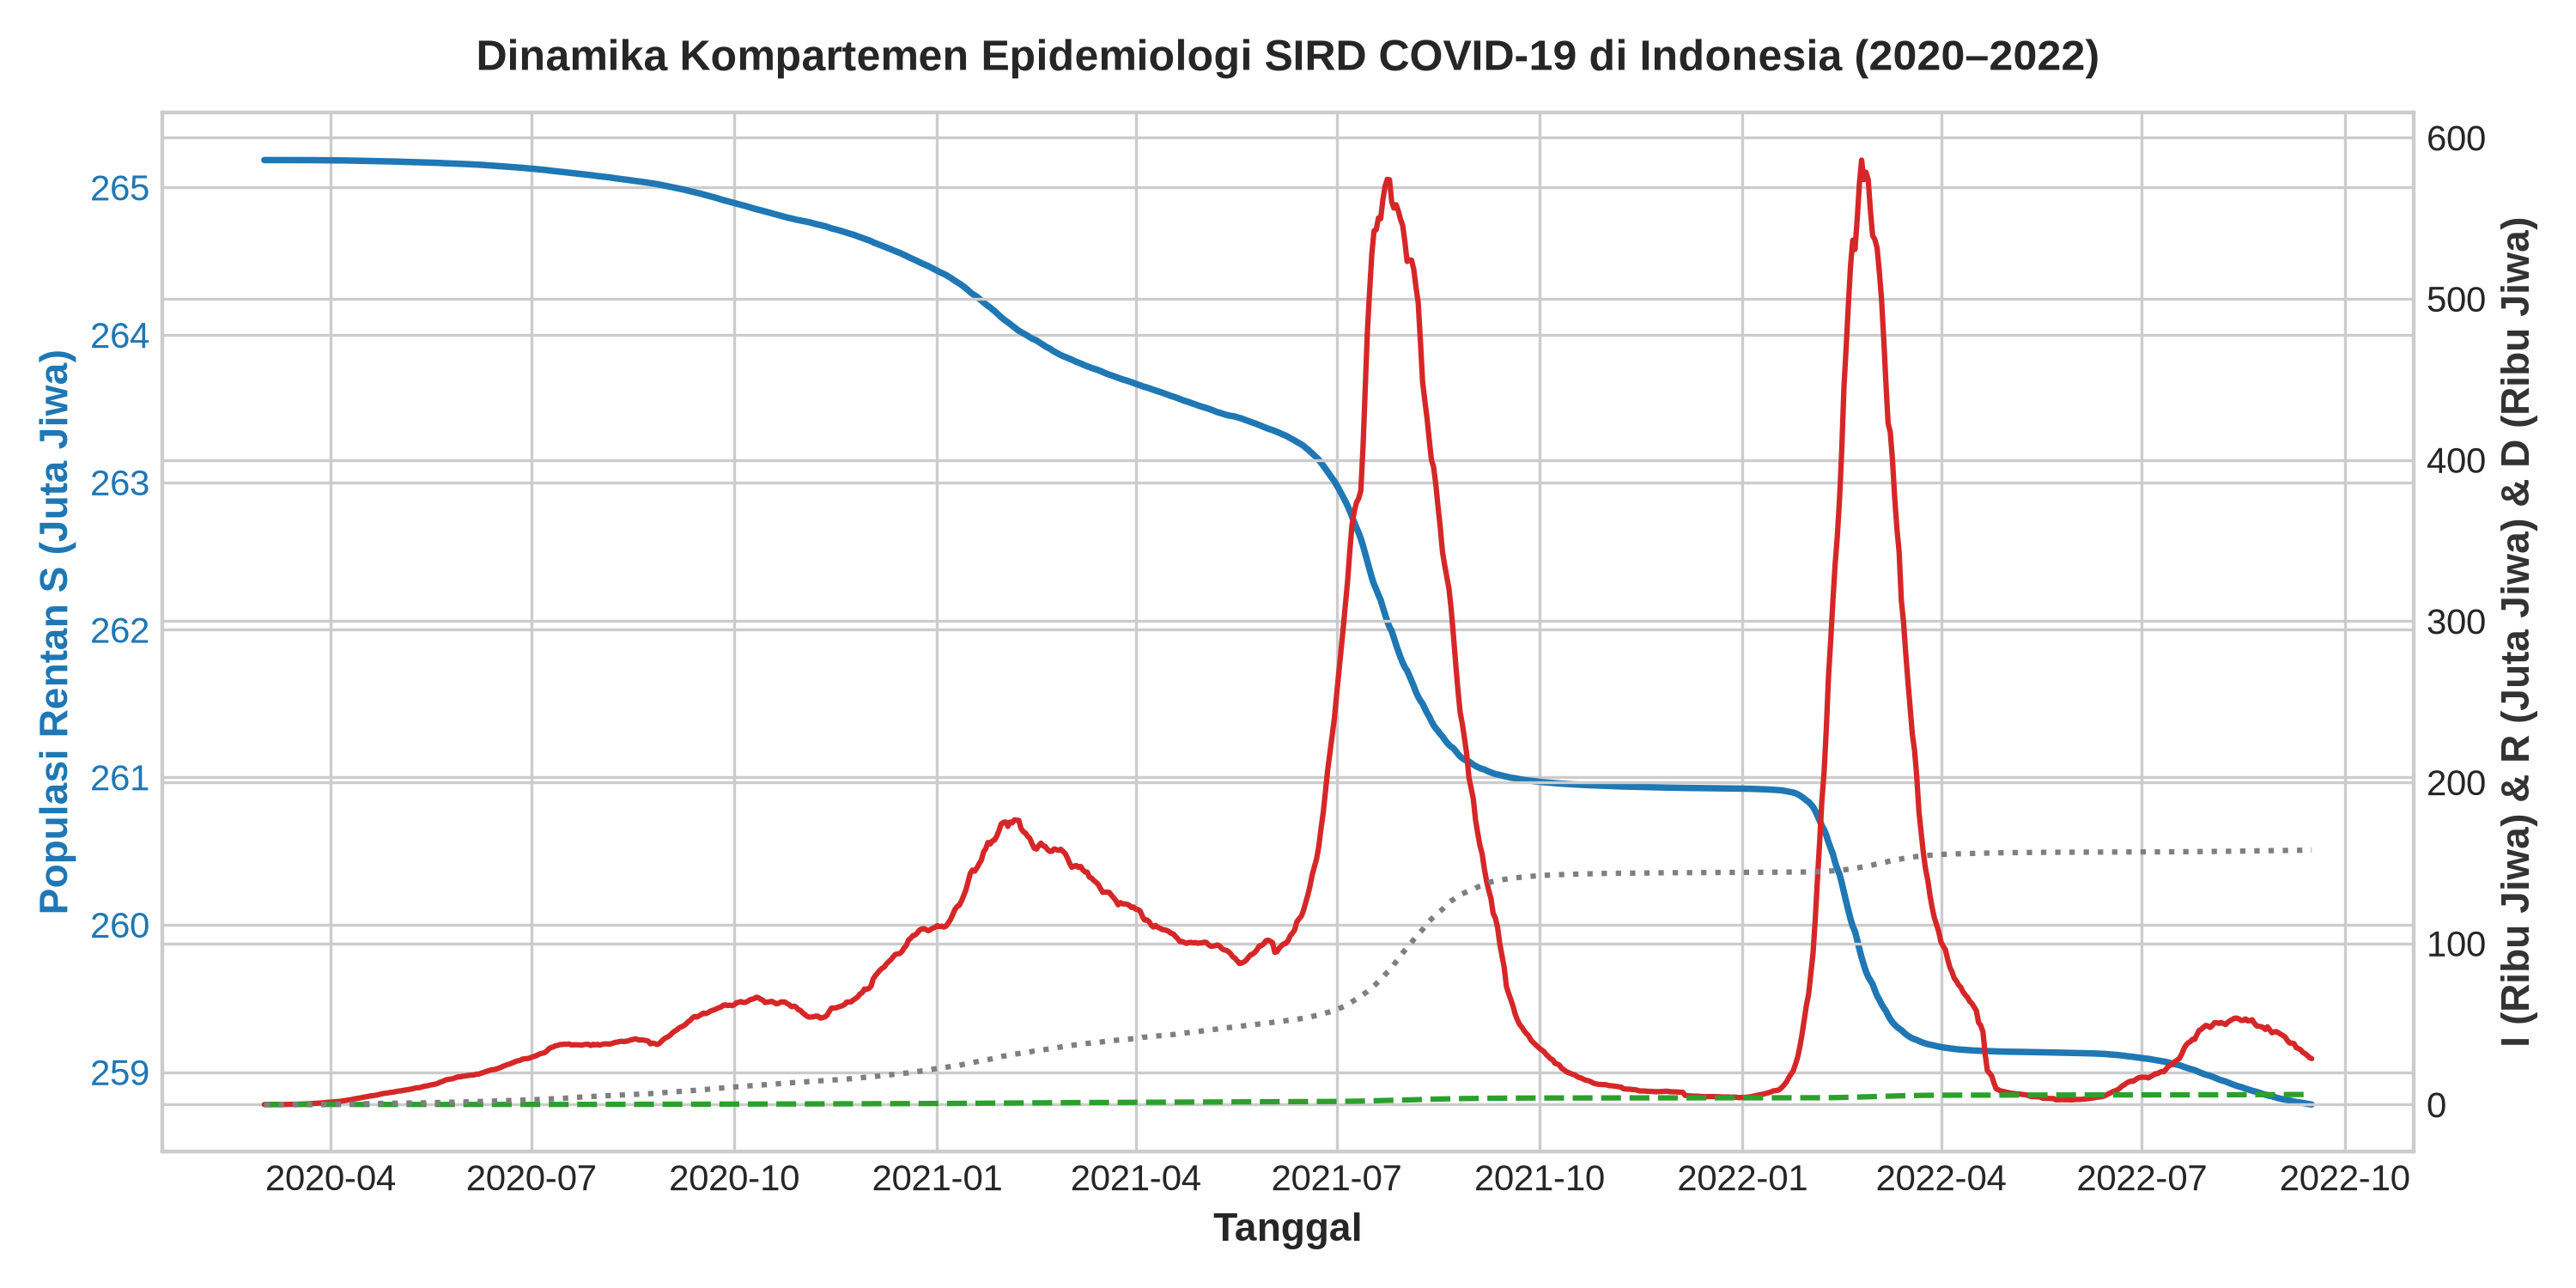
\includegraphics[width=0.92\textwidth]{figures/dinamika_sird_indonesia.png}
  \caption{Dinamika Runtut Waktu Kompartemen SIRD COVID-19 di Indonesia (Maret 2020 hingga September 2022)}
  \label{fig:dinamika_sird}
\end{figure}

\begin{figure}[H]
  \centering
  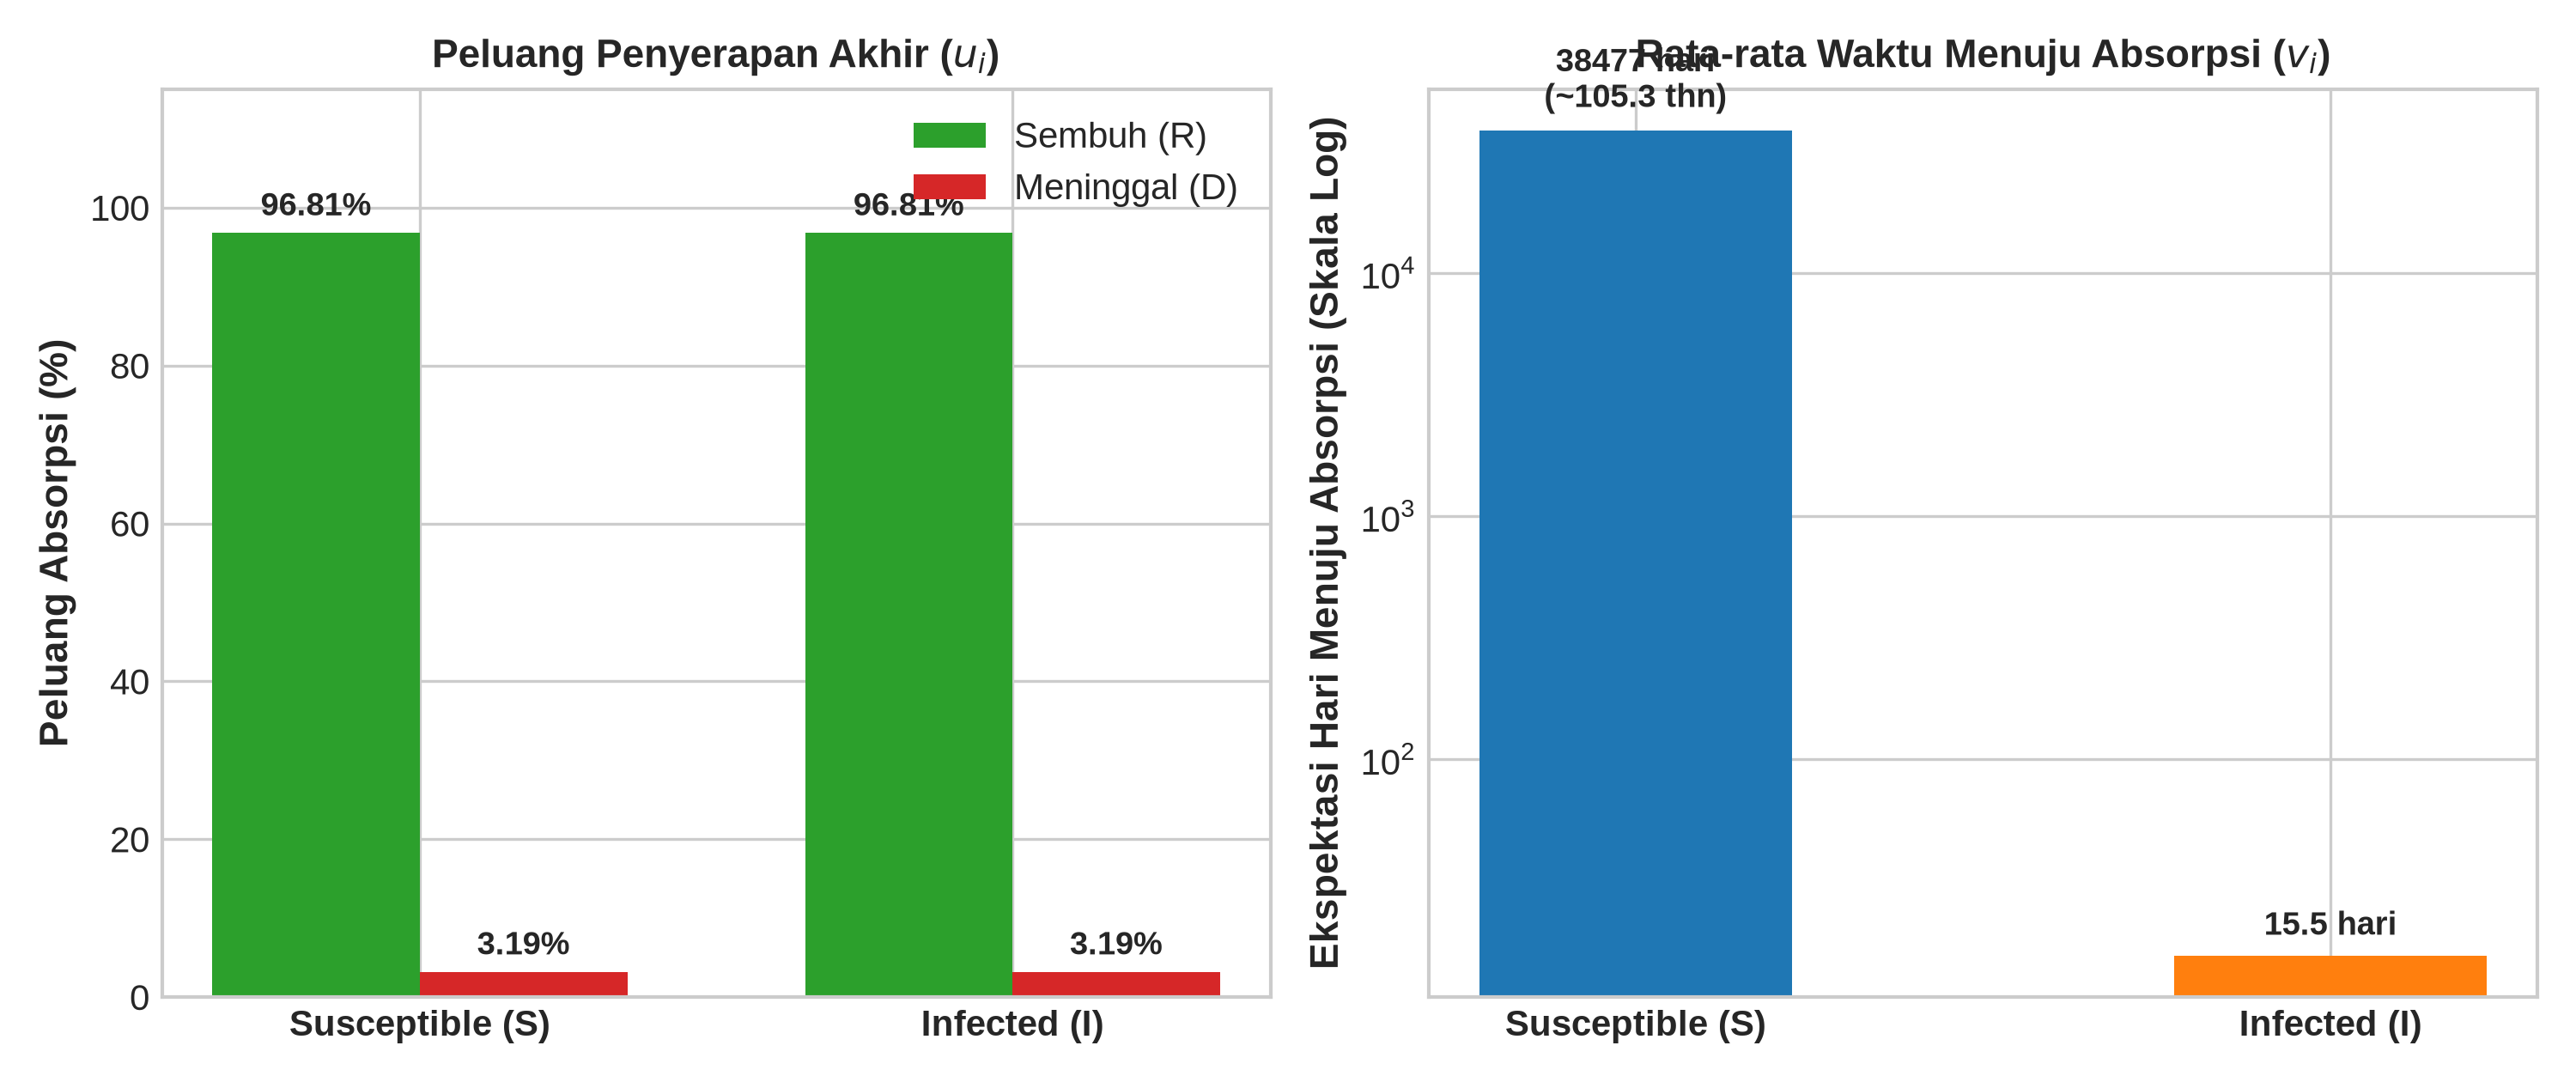
\includegraphics[width=0.92\textwidth]{figures/hasil_fsa_sird.png}
  \caption{Hasil Analisis Langkah Pertama: (Kiri) Peluang Penyerapan Akhir ($u_i$), (Kanan) Waktu Rata-rata Menuju Penyerapan ($v_i$)}
  \label{fig:hasil_fsa}
\end{figure}

\end{document}
